\begin{figure}[t]
    \centering
    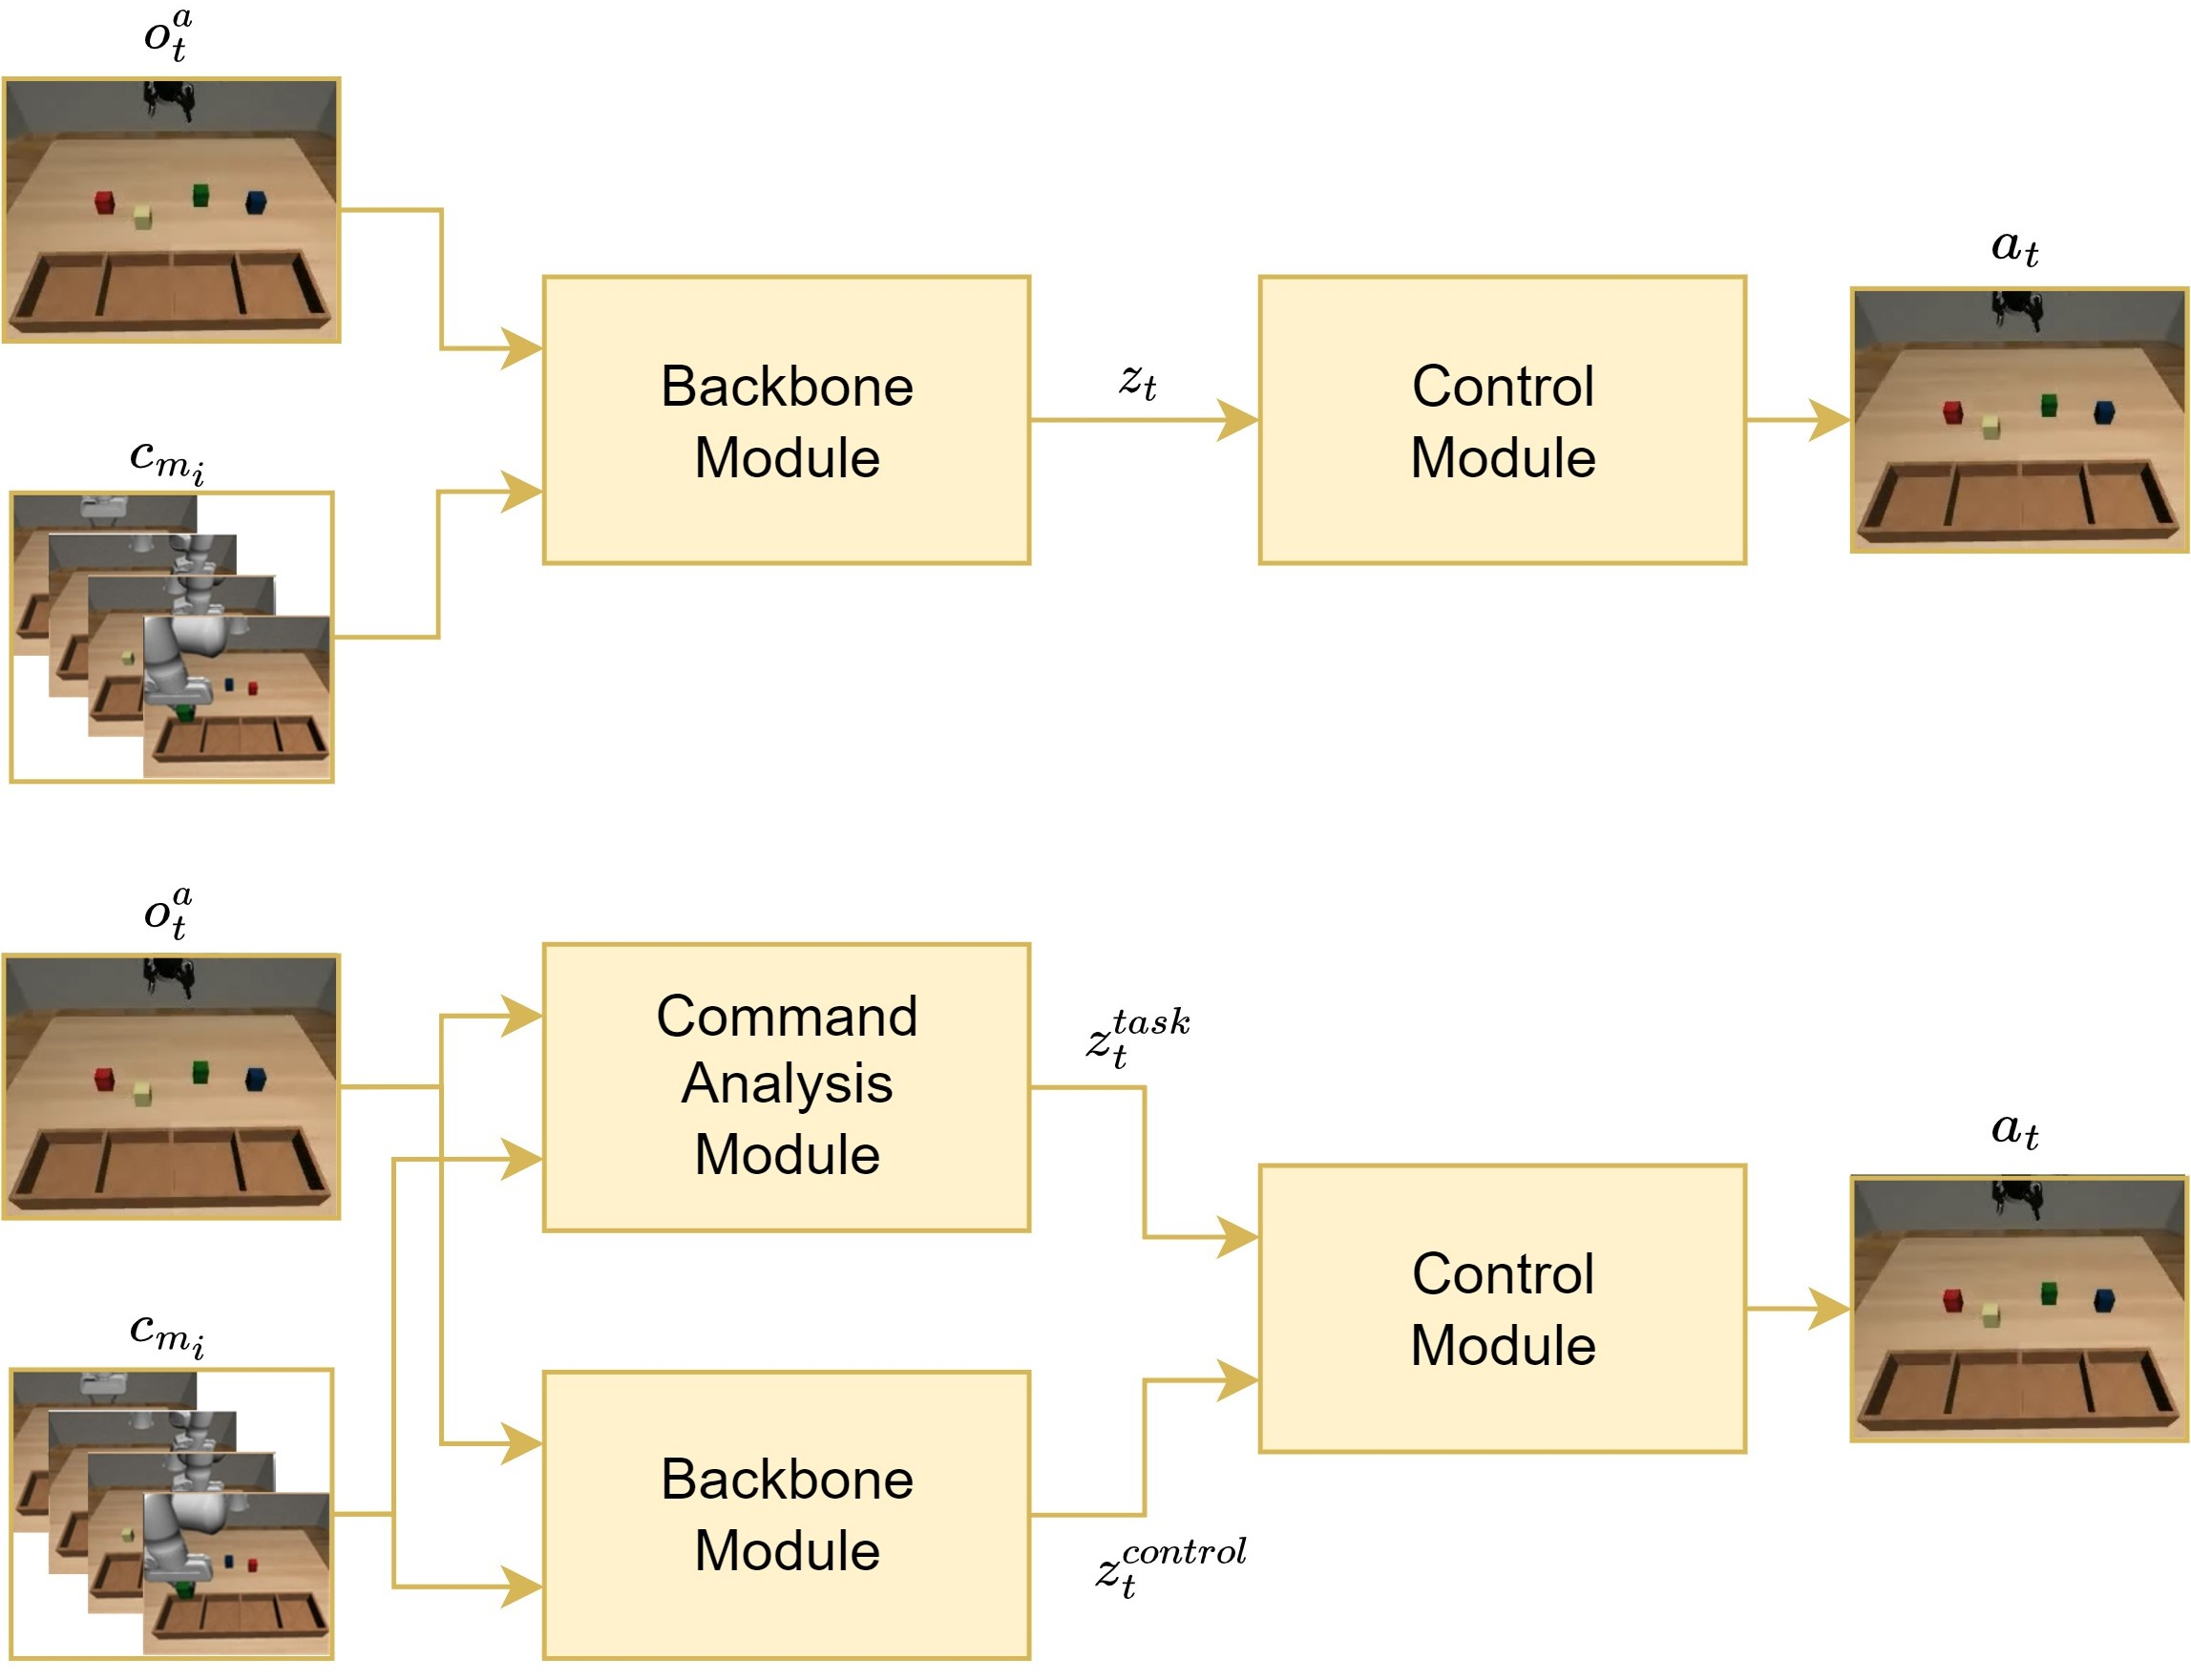
\includegraphics[width=0.7\textwidth]{figures/images/ch3/end_to_end_vs_modular.jpg}
    \caption{(Upper) General end-to-end architecture, where the \textit{Backbone Module} takes as input both the agent observation and the command. It generates an embedding $z_{t}$ that must contain information related to both the command and the control. (Bottom) In the modular architecture, there are two backbone modules: the \textit{Command Analysis Module}, which generates the task-embedding $z^{task}_t$, and the \textit{Backbone Module}, which is trained to generate only the control-embedding $z^{control}_{t}$.}
    \label{fig:end_to_end_vs_modular}
\end{figure}
